% Tutorial set: 04
% Source: Tutorial 4, Deep neural networks, Questions 1--3
% Reference: Tutorial 4 reference solutions, PDF pages 1--43
% Session date: 2026-09-09
% Human verified: Yes; formula, preprocessing, baseline, and reference-figure issues corrected

\subsection{Tutorial 04：Deep Network Backpropagation、Softmax 与 Integrated Gradients}
\label{tutorial:SC4001-TUT04}

\exercisemeta
  {SC4001-TUT04}
  {2026-09-09}
  {Tutorial 4：Deep neural networks，Questions 1--3；官方参考解答用于核对}
  {三题已完成；订正 SGD 导数记号、data leakage、Softmax 实现、IG baseline 与参考图不一致}
  {已确认（2026-09-09）}

\exercisequestion{SC4001-TUT04-Q01}{Two-layer Sigmoid Network：GD、SGD 与 Backpropagation}

\textbf{对应讲义：}
\relatedtopic{SC4001-L04-T01}{Chain Rule 与 Computational Graph}；\par\noindent
\relatedtopic{SC4001-L04-T02}{Two-layer FFN：Single-sample Backpropagation}；\par\noindent
\relatedtopic{SC4001-L04-T03}{Batch Backpropagation 与 Shape Check}

\subsubsection*{题目}

Two-input, two-hidden, two-output network（双输入、双隐藏、双输出网络）的两个 layers（层）均使用 sigmoid：
\[
  \bm W=\begin{bmatrix}1&2\\-2&0\end{bmatrix},\quad
  \bm b=\begin{bmatrix}3&-1\end{bmatrix},\quad
  \bm V=\begin{bmatrix}1&1\\0&-2\end{bmatrix},\quad
  \bm c=\begin{bmatrix}-2&3\end{bmatrix}.
\]
训练数据与 targets（目标）为
\[
  \bm X=\begin{bmatrix}1&3\\-2&-2\end{bmatrix},\qquad
  \bm D=\begin{bmatrix}0&1\\1&0\end{bmatrix}.
\]
使用 $\alpha=0.05$，完成一次 full-batch GD（全批量梯度下降）及 SGD（随机梯度下降），并训练至 convergence（收敛）。

\begin{checkedsolution}
Batch forward propagation（批量前向传播）为
\[
  \bm Z=\bm X\bm W+\bm1\bm b
  =\begin{bmatrix}-2&1\\5&-5\end{bmatrix},\qquad
  \bm H=\sigma(\bm Z)
  \approx\begin{bmatrix}0.119&0.731\\0.993&0.007\end{bmatrix},
\]
\[
  \bm U=\bm H\bm V+\bm1\bm c
  \approx\begin{bmatrix}-1.881&1.657\\-1.007&3.980\end{bmatrix},\qquad
  \bm Y=\sigma(\bm U)
  \approx\begin{bmatrix}0.132&0.840\\0.268&0.982\end{bmatrix}.
\]
按参考解答的 square-error convention（平方误差约定），
\[
  J=\frac12\sum_{p,k}(d_{pk}-y_{pk})^2\approx0.7716.
\]

令 $\bm\Delta_U=\nabla_{\bm U}J$、$\bm\Delta_Z=\nabla_{\bm Z}J$。Chain rule（链式法则）给出
\[
  \boxed{\bm\Delta_U=(\bm Y-\bm D)\odot\bm Y\odot(1-\bm Y)},
\]
\[
  \boxed{\bm\Delta_Z=(\bm\Delta_U\bm V^{\mathsf T})
  \odot\bm H\odot(1-\bm H)}.
\]
数值上
\[
  \bm\Delta_U\approx
  \begin{bmatrix}0.0152&-0.0215\\-0.1435&0.0177\end{bmatrix},\qquad
  \bm\Delta_Z\approx
  \begin{bmatrix}-0.00067&0.00847\\-0.00084&-0.00024\end{bmatrix}.
\]
其中 $\bm\Delta_U\bm V^{\mathsf T}$ 把所有 downstream gradients（下游梯度）按连接权重汇总到每个 hidden neuron（隐藏神经元）；随后还要乘该 neuron 自身的 sigmoid derivative（Sigmoid 导数）。

Parameter gradients（参数梯度）为
\[
  \nabla_{\bm V}J=\bm H^{\mathsf T}\bm\Delta_U,\quad
  \nabla_{\bm c}J=\bm\Delta_U^{\mathsf T}\bm1,\quad
  \nabla_{\bm W}J=\bm X^{\mathsf T}\bm\Delta_Z,\quad
  \nabla_{\bm b}J=\bm\Delta_Z^{\mathsf T}\bm1.
\]
一次 GD update（更新）后
\[
  \bm V'\approx\begin{bmatrix}1.0070&0.9993\\-0.0005&-1.9992\end{bmatrix},\quad
  \bm c'\approx\begin{bmatrix}-1.9936&3.0002\end{bmatrix},
\]
\[
  \bm W'\approx\begin{bmatrix}1.0000&1.9996\\-2.0000&-0.0013\end{bmatrix},\quad
  \bm b'\approx\begin{bmatrix}3.0001&-1.0004\end{bmatrix}.
\]

参考运行的 GD convergence result（收敛结果）约为
\[
  \bm W=\begin{bmatrix}0.63&0.60\\-3.00&-2.00\end{bmatrix},\quad
  \bm b=\begin{bmatrix}2.72&-0.74\end{bmatrix},
\]
\[
  \bm V=\begin{bmatrix}4.97&-3.46\\0.25&-2.37\end{bmatrix},\quad
  \bm c=\begin{bmatrix}-2.42&2.56\end{bmatrix},\quad
  \bm Y\approx\begin{bmatrix}0.08&0.94\\0.93&0.05\end{bmatrix}.
\]
参考页报告 GD MSE $0.0089$、SGD MSE $0.004$；两组 parameters 只在显示到两位小数时相同，不能据此认为 non-convex training（非凸训练）必然得到同一组参数。

GD 用同一组旧 parameters 计算整个 batch 后才更新；SGD 处理第一个 pattern 后立即更新，第二个 pattern 必须使用更新后的 parameters。参考答案的 SGD 总公式把 output derivative 写成 $f'(\bm z)$，这是 notation typo（记号笔误），应为 $f'(\bm u)$。此外，$z=\pm5$ 时 sigmoid 已接近饱和，$\sigma'(z)$ 很小，因此隐藏层容易出现 vanishing gradient（梯度消失）。
\end{checkedsolution}

\exercisequestion{SC4001-TUT04-Q02}{Three-class Network：Softmax、Cross-entropy 与 Decision Regions}

\textbf{对应讲义：}
\relatedtopic{SC4001-L03-T04}{Softmax、Cross-entropy 与 Logit Gradient}；
\relatedtopic{SC4001-L03-T05}{Softmax Decision Boundaries}；
\relatedtopic{SC4001-L04-T03}{Batch Backpropagation 与 Shape Check}

\subsubsection*{题目}

六个 two-dimensional samples（二维样本）属于 A、B、C 三类：
\[
  A:(1,1),(0,1),\qquad
  B:(3,4),(2,2),\qquad
  C:(2,-2),(-2,-3).
\]
网络采用 three-neuron sigmoid hidden layer（三神经元 Sigmoid 隐藏层）与 three-neuron Softmax output（三神经元 Softmax 输出层），初值为
\[
  \bm W=\begin{bmatrix}-0.10&0.97&0.18\\-0.70&0.38&0.93\end{bmatrix},\quad
  \bm b=\bm0,
\]
\[
  \bm V=\begin{bmatrix}
    1.01&0.09&-0.39\\0.79&-0.45&-0.22\\0.28&0.96&-0.07
  \end{bmatrix},\quad \bm c=\bm0,\qquad \alpha=0.1.
\]
要求完成一次 GD、训练至收敛、预测两个新样本，并在 $[-4,4]^2$ 上画出 decision regions（决策区域）。

\begin{checkedsolution}
令 $\bm K$ 为 one-hot target matrix（独热目标矩阵）。初始 forward pass 得到
\[
  \bm P\approx
  \begin{bmatrix}
    0.59&0.28&0.13\\0.54&0.31&0.15\\0.56&0.31&0.14\\
    0.58&0.29&0.13\\0.73&0.16&0.11\\0.59&0.25&0.16
  \end{bmatrix}.
\]
每行 maximum probability（最大概率）都在第一列，所以初始模型把六个样本全判为 class A，错误数为 $4$，cross-entropy（交叉熵）约为 $7.63$。Softmax 与 cross-entropy 组合后
\[
  \boxed{\nabla_{\bm U}J=\bm P-\bm K}.
\]
一次更新的主要结果为
\[
  \bm W'\approx\begin{bmatrix}-0.13&0.95&0.18\\-0.63&0.42&0.95\end{bmatrix},\quad
  \bm b'\approx\begin{bmatrix}-0.02&0&-0.01\end{bmatrix},
\]
\[
  \bm V'\approx\begin{bmatrix}0.92&0.05&-0.26\\0.68&-0.36&-0.19\\0.22&1.05&-0.10\end{bmatrix},\quad
  \bm c'\approx\begin{bmatrix}-0.16&0.04&0.12\end{bmatrix}.
\]

参考运行在收敛时给出
\[
  \bm W\approx\begin{bmatrix}-1.81&0.32&0.08\\-1.40&2.92&1.91\end{bmatrix},\quad
  \bm b\approx\begin{bmatrix}4.36&0.73&-1.71\end{bmatrix},
\]
\[
  \bm V\approx\begin{bmatrix}
    2.93&-5.33&3.12\\2.80&1.20&-3.87\\0.09&4.55&-3.47
  \end{bmatrix},\quad
  \bm c\approx\begin{bmatrix}-1.94&-0.06&2.01\end{bmatrix}.
\]
六个 training labels（训练标签）全部正确。两个 test patterns（测试样本）的结果为
\[
  (2.5,1.5)\mapsto(0.05,0.95,0.00)\mapsto B,\qquad
  (-1.5,0.5)\mapsto(0.93,0.00,0.07)\mapsto A.
\]

\begin{figure}[htbp]
  \centering
  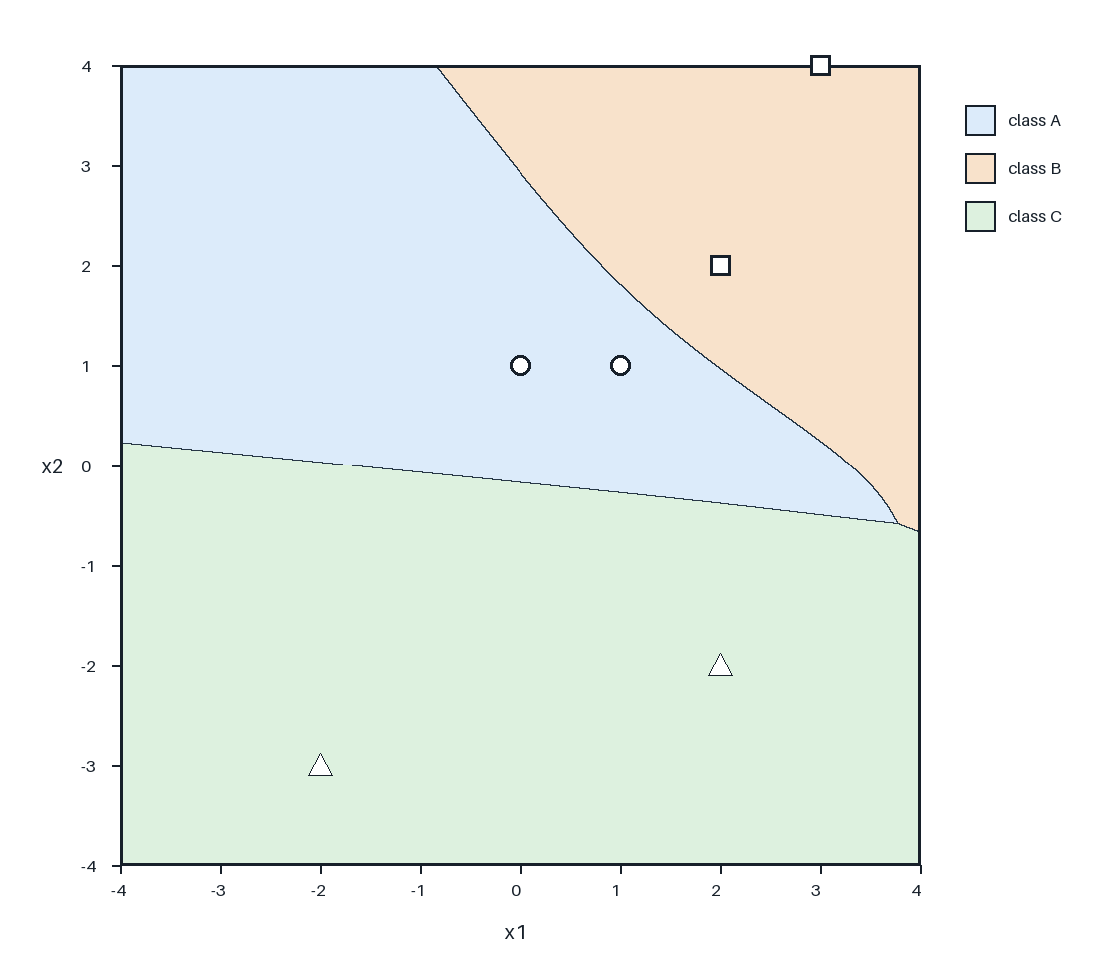
\includegraphics[width=0.72\textwidth]{figures/source/tutorial-04-q2-decision-regions.png}
  \caption{由官方参考解答 PDF p.~31 公布的收敛参数重新计算的 decision regions。参考解答 p.~33 的原图与其参数及 training labels 不一致，故未直接采用；本图同时标出六个训练样本并验证其预测均正确。}
  \label{fig:sc4001-tut04-decision-regions}
\end{figure}

Hidden sigmoid（隐藏层 Sigmoid）使 $\bm h=\sigma(\bm x\bm W+\bm b)$ 成为 nonlinear feature map（非线性特征映射），因此原输入空间中可以出现 nonlinear boundaries。若移除全部 nonlinear activations（非线性激活），则
\[
  (\bm X\bm W+\bm B)\bm V+\bm C
  =\bm X(\bm W\bm V)+(\bm B\bm V+\bm C),
\]
多层 linear maps（线性映射）仍等价于一层 linear map，不能增加 decision-boundary complexity（决策边界复杂度）。
\end{checkedsolution}

\exercisequestion{SC4001-TUT04-Q03}{Titanic Classification 与 Integrated Gradients}

\textbf{对应讲义：}
\relatedtopic{SC4001-L04-T04}{General DNN：逐层递推的 Backpropagation}；
\relatedtopic{SC4001-L04-T05}{Preprocessing、Width、Depth 与 Parameter Count}

\subsubsection*{题目}

对 Titanic dataset（泰坦尼克数据集）完成 categorical one-hot encoding（类别独热编码）、missing-value imputation（缺失值填充）、feature selection（特征选择）及 $70{:}30$ train/test split。训练
\[
  12\rightarrow12\rightarrow8\rightarrow2
\]
的 classifier（分类器）：两个 hidden layers 使用 sigmoid，输出对应 survived/not survived；optimizer 为 Adam，$\alpha=0.1$，训练 200 epochs。最后使用 Captum 的 Integrated Gradients（积分梯度）解释 input-feature importance（输入特征重要性）。题目原文将本组误编号为第二题，此处按内容记为 Q3。

\begin{checkedsolution}
十二个 inputs 为
\[
  \underbrace{\texttt{age,sibsp,parch,fare}}_{4\text{ numerical}}
  +\underbrace{\texttt{female,male}}_{2}
  +\underbrace{\texttt{embark\_C/Q/S}}_{3}
  +\underbrace{\texttt{class\_1/2/3}}_{3}.
\]
One-hot encoding 避免把 nominal categories（名义类别）错误解释成具有固定数值距离。严格的无泄漏流程应先 split，再只用 training set 估计 age/fare means，并用这些 training statistics 同时填充 train 与 test；参考代码先在完整 dataset 上求均值，会造成 data leakage（数据泄漏）。

参考运行报告
\[
  \text{training accuracy}=84.72\%,\qquad
  \text{test accuracy}=81.68\%.
\]
单次随机 split 不足以稳定判断 generalization（泛化）。若 PyTorch 使用 \texttt{CrossEntropyLoss}，network 应返回 raw logits（原始逻辑值），因为该 loss 已内置 \texttt{log\_softmax}；不应把显式 \texttt{Softmax} 的结果再次输入它。

对目标输出 $F(x)$、真实输入 $x$ 与 baseline（基准输入）$x'$，第 $i$ 个 Integrated Gradient 为
\[
  IG_i(x)=(x_i-x_i')\int_0^1
  \frac{\partial F\!\left(x'+\alpha(x-x')\right)}{\partial x_i}\,d\alpha.
\]
参考代码调用 \texttt{target=1} 表示解释 survived output（生存输出）；它没有传入 \texttt{baselines}，所以 Captum 默认使用 twelve-dimensional all-zero input（十二维全零输入）。两者不能混淆。

对 survived output 的平均 attributions（归因）为：
\begin{center}
\small
\begin{tabular}{@{}lrlr@{}}
  \toprule
  Feature & Attribution & Feature & Attribution \\
  \midrule
  age & $-0.397$ & sibsp & $-0.063$ \\
  parch & $-0.012$ & fare & $+0.074$ \\
  female & $+0.116$ & male & $-0.432$ \\
  embark\_C & $+0.112$ & embark\_Q & $+0.020$ \\
  embark\_S & $-0.087$ & class\_1 & $+0.075$ \\
  class\_2 & $+0.016$ & class\_3 & $-0.144$ \\
  \bottomrule
\end{tabular}
\end{center}
符号表示相对于所选 baseline，feature 将 survived output 推高或压低；数值不是概率变化百分比，更不是 causal effect（因果效应）。默认 baseline 中 \texttt{female=male=0} 且三个 class indicators 全为 0，并不对应 valid passenger（合法乘客），所以解释语义较弱。更合理的选择包括 training mean、明确的 reference passenger（参考乘客）或多个 baselines 的平均；改变 baseline 会改变 attribution。
\end{checkedsolution}

\subsubsection*{本次 Tutorial 收口}

Q1 把 chain rule 落到 two-layer GD/SGD，并暴露 sigmoid saturation 与 vanishing gradient；Q2 将 hidden nonlinear features、Softmax、cross-entropy 和 nonlinear decision regions 连成一条完整分类流程；Q3 强调 preprocessing statistics、PyTorch loss interface 与 attribution baseline 都是模型定义的一部分。复现结果时不能只记录 weights，还必须记录 loss convention、update order、data split、preprocessing 和解释基准。
